\documentclass[twoside,a4paper]{article}
\usepackage{geometry}
\geometry{margin=1.5cm, vmargin={0pt,1cm}}
\setlength{\topmargin}{-1cm}
\setlength{\paperheight}{29.7cm}
\setlength{\textheight}{25.3cm}

% useful packages.
\usepackage{float}
\usepackage{tikz}
\usetikzlibrary{calc}
\usetikzlibrary{arrows.meta}
\usepackage{pgfplots}
\usepackage{amsfonts}
\usepackage{amsmath}
\usepackage{amssymb}
\usepackage{amsthm}
\usepackage{enumerate}
\usepackage{graphicx}
\usepackage{multicol}
\usepackage{fancyhdr}
\usepackage{layout}
\usepackage{listings}
\usepackage{longtable}
\usepackage{multirow}
\usepackage{graphicx}
\usepackage{subfigure} 

% some common command
\newcommand{\dif}{\mathrm{d}}
\newcommand{\avg}[1]{\left\langle #1 \right\rangle}
\newcommand{\difFrac}[2]{\frac{\dif #1}{\dif #2}}
\newcommand{\pdfFrac}[2]{\frac{\partial #1}{\partial #2}}
\newcommand{\OFL}{\mathrm{OFL}}
\newcommand{\UFL}{\mathrm{UFL}}
\newcommand{\fl}{\mathrm{fl}}
\newcommand{\op}{\odot}
\newcommand{\Eabs}{E_{\mathrm{abs}}}
\newcommand{\Erel}{E_{\mathrm{rel}}}
\begin{document}

\tikzset{
  dot/.style={
    circle, fill=black, inner sep=1pt, outer sep=0pt
  },
  dot label/.style={
    circle, inner sep=0pt, outer sep=1pt
  }
  arrow1/.style = {
    draw = black, thick, -{Latex[length = 4mm, width = 1.5mm]},
  }
}

\pagestyle{fancy}
\fancyhead{}
\lhead{Liu jiyu (3170104256)}
\chead{Design Document}
\rhead{2021.1}

Our goal is to design a program, whose input is several sets of coordinates
of the points, which can represent a Yin set, the program provides the
function to determine the complement,intersection and regularized
union of the Yin sets.

As we know, Yin set is uniquely represented by a realizable spajor, a
spajor is the union of a finite number of atom spadjors. An atom
spajor is the union of finite number of Jordan Curves. For Jordan
curves, we can approximate with linear polygons, i.e. we can represent
a Jordan curve with a finite number of segments. So we have a
fundamental thought for designing class:

$$
\mbox{Point}\rightarrow\mbox{Segment}\rightarrow\mbox{Jordan\_Curve}
\rightarrow\mbox{Atom\_Spajor}\rightarrow\mbox{Spajor}
$$

The arrow means the right part consists of finite number of the left
parts, it is a has-a relation. So we can let a vector of left part be
a member of a class of the right part.

The final goal is to implement the algorithm of complement, meet and
join, whose input is a spajor or two spajors.

Firstly, according to the algorithm of complement, we need three
functions, Cut,Pasting and Reverse.

For Cut function, we need to traverse the Jordan Curves of the spajor
and determine the relative position of the point and each segment of the
Jordan Curve and cut the Jordan Curve, so we have to implement the
judgement in class Segment and cut function in class Jordan\_Curve for
reusing . To implement it , we also need a function to calculate the slope of the
segment.

For Pasting function, for a fixed point v, we will find the edges whose
starting point or ending point is v, so we can write functions
Find\_in, Find\_out for reusing. Similarly, for a fixed edge, we will
also find the edge of which the positive counterclockwise angle is the
smallest. So we will write the function MinAngleEdge, which also needs
a function to calculate this angle in Class Segment, which we can call
it Angle(). In the algorithm of pasting function, we also have S2R-c
conditions, which tells that we may get a wrong curve which consists
of two or more Jordan curves, so we have to write a function to judge
whether a curve is Jordan\_Curve and get all self-intersections of this
curve,which can be implemented in class Jordan\_Curve.

Implementing Reverse Function is easy in Class Segment. When we
implement these functions, the complementation is 
almost completed.

\vbox{}
For Meet function, the first thing we have to do is to get the point
set V and the segment set E.

To get V, we have to get the
intersections of two spajors, which we can reduce it to judge whether
two curves or two segments or a curve and a segment intersect, and
further get the intersections of two curves, the intersections of a
curve and a segment, and the intersections of two segments.

To get E, we have to judge whether a edge is in the interior of the
spajor or it is just a edge of the spajor, the latter is easy and the
former is non-trivial. So we have to use
Atom\_Spajor, as we know an atom spajor represents a connected Yin set,
we can reduce this problem to judge whether a segment is in the Yin
set represented by a atom\_spajor, which is related to the relative
position of a segment and a Jordan Curve. So we can reduce it futher
to judge a segment is in the interior of the Jordan Curve. To
implement it, we can firstly judge whether the segment is in the
bounded components of the Jordan curve's complementation,which we can also
reduce it further to judge whether a point is in the bounded
components of the Jordan curve's complementation. We call all these
functions for judging "include" relation IsInclude(), then we can get
Ori\_IsInclude() to complete our goal.

Then the meet function is almostly completed, and the join function
can be easily deduced from meet function and complement function.

By the way, when we implement the IsInclude() function, we have to use
the relative position of two segments, so we can write some functions
to determine it.

When we integrate these functions in their "home", we will have a
clear thought to achieve our final goal.


The following is the UML picture of design thought:

\begin{figure}[H]
  \begin{center}
  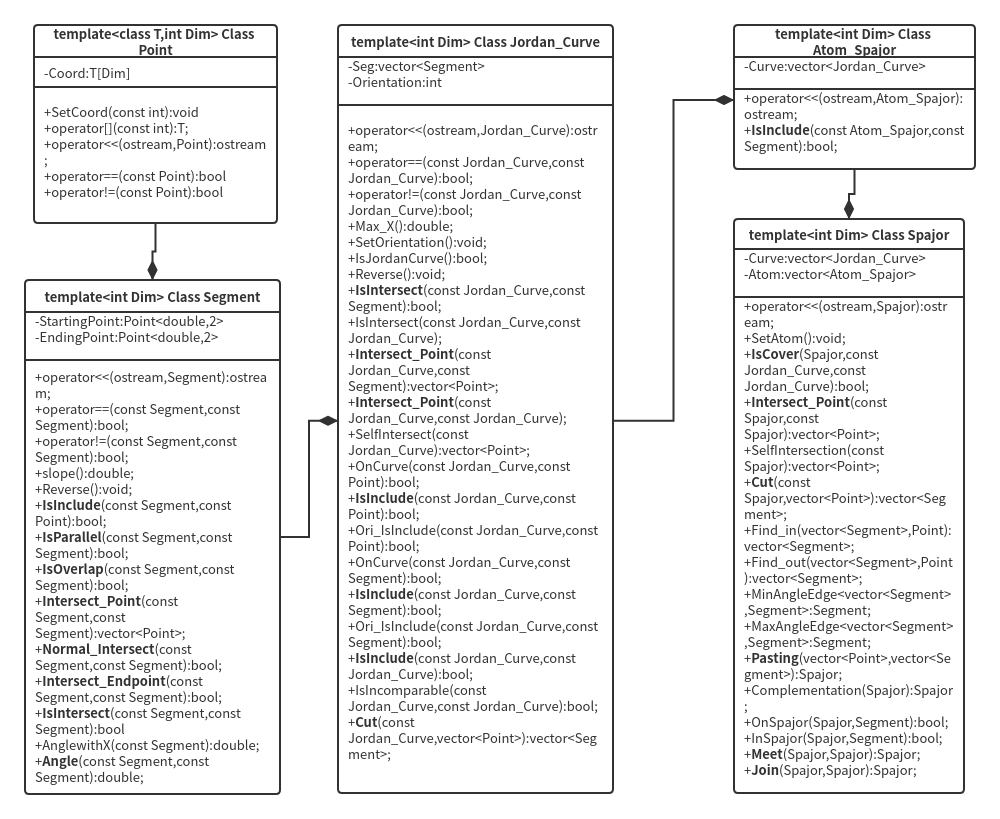
\includegraphics[height=15cm]{./pic/UML.png}
  \caption{UML picture}
  \end{center}
  \label{fig:figure1}
\end{figure}

\newpage

For class Segment, I write all possible positions of two segments,
some of which may not be used in the whole program. But it may be
useful when we have some other goals.

As the above has-a relation diagram, the latter class will reuse the
functions of the former class for many many times, so the project
avoids the useless repeating.

There are also some places in the program, such as I can put all these position
judging functions and functions for intersections into the class and
use the template specialization to implement the two-dimension
condition. What's more, there are some more efficient algorithm to
implement some functions, such as scan line algorithm for calculating
the intersections of two linear polygons.

\end{document}
%%% Local Variables:
%%% mode: latex
%%% TeX-master: t
%%% End:
